\documentclass[]{article}

\usepackage{lmodern}
\usepackage{amssymb,amsmath,amsfonts,amsthm}
\usepackage{ifxetex,ifluatex}
\usepackage{fixltx2e} % provides \textsubscript
\DeclareMathOperator*{\argmin}{arg\,min}
\ifnum 0\ifxetex 1\fi\ifluatex 1\fi=0 % if pdftex
  \usepackage[T1]{fontenc}
  \usepackage[utf8]{inputenc}
\else % if luatex or xelatex
  \ifxetex
    \usepackage{mathspec}
  \else
    \usepackage{fontspec}
  \fi
  \defaultfontfeatures{Ligatures=TeX,Scale=MatchLowercase}
  \newcommand{\euro}{€}
\fi
% use upquote if available, for straight quotes in verbatim environments
\IfFileExists{upquote.sty}{\usepackage{upquote}}{}
% use microtype if available
\IfFileExists{microtype.sty}{%
\usepackage{microtype}
\UseMicrotypeSet[protrusion]{basicmath} % disable protrusion for tt fonts
}{}
\usepackage{hyperref}
\PassOptionsToPackage{usenames,dvipsnames}{color} % color is loaded by hyperref
\hypersetup{unicode=true,
            pdftitle={Generating Precise Ad Targeting Hypotheses for Scalable Testing},
            colorlinks=true,
            linkcolor=blue,
            citecolor=blue,
            anchorcolor=blue,
            urlcolor=blue,
            breaklinks=true}
\urlstyle{same}  % don't use monospace font for urls
\usepackage[backend=bibtex,style=numeric,hyperref=true,backref=true,maxnames=99]{biblatex}
\addbibresource{mybib.bib}
\usepackage{graphicx,grffile}
\usepackage{tabularx}
\usepackage{makecell}
\usepackage{changepage}
\usepackage{caption}
\makeatletter
\def\maxwidth{\ifdim\Gin@nat@width>\linewidth\linewidth\else\Gin@nat@width\fi}
\def\maxheight{\ifdim\Gin@nat@height>\textheight\textheight\else\Gin@nat@height\fi}
\makeatother
% Scale images if necessary, so that they will not overflow the page
% margins by default, and it is still possible to overwrite the defaults
% using explicit options in \includegraphics[width, height, ...]{}
\setkeys{Gin}{width=\maxwidth,height=\maxheight,keepaspectratio}
\setlength{\parindent}{0pt}
\setlength{\parskip}{6pt plus 2pt minus 1pt}
\setlength{\emergencystretch}{3em}  % prevent overfull lines
\providecommand{\tightlist}{%
  \setlength{\itemsep}{0pt}\setlength{\parskip}{0pt}}
\setcounter{secnumdepth}{5}

%\usepackage{caption}
%\renewcommand{\captionfont}{\small} %small fonts for caption
%\renewcommand{\captionlabelfont}{\small}

% \usepackage{url}
% \usepackage{balance}

%% Adding URL breaks
% \makeatletter
% \g@addto@macro{\UrlBreaks}{\UrlOrds}
% \makeatother

% \usepackage{lastpage}

%\usepackage[aboveskip=2pt]{subcaption} %for subfigures

%\setlength{\textfloatsep}{0pt} %spacing between figures and texts
%\setlength{\floatsep}{0pt} 
%\setlength{\dblfloatsep}{0pt}
%\setlength{\dbltextfloatsep}{0pt}
%\setlength{\abovecaptionskip}{0pt}
%\renewcommand{\footnotesize}{\scriptsize}

%\usepackage{etoolbox} % spacing between formula and text
%\apptocmd\normalsize{%
%\abovedisplayskip=0pt
%\abovedisplayshortskip=0pt
%\belowdisplayskip=0pt
%\belowdisplayshortskip=0pt
%}{}{}

%\let\oldfootnote\footnote %small footnote
%\renewcommand{\footnote}[1]{{\oldfootnote{\scriptsize #1}}}

%%% Macros for convenience
%% References
\newcommand{\secref}[1]{\S\ref{sec:#1}}
\newcommand{\figref}[1]{Figure~\ref{fig:#1}}
\newcommand{\tabref}[1]{Table~\ref{tab:#1}}

%% Common latin terms
\newcommand{\etc}{\emph{etc.}\xspace}
\newcommand{\ie}{\emph{i.e.,}\xspace}
\newcommand{\eg}{\emph{e.g.,}\xspace}
\newcommand{\etal}{\emph{et al.}\xspace}

%%%%% Squeezing space before sections, subsections, and re-defining
%%%%% paragraphs
\makeatletter
\let\origsection\section
\let\origsubsection\subsection
\let\origparagraph\paragraph

\renewcommand\section{\@ifstar{\starsection}{\nostarsection}}
\renewcommand\subsection{\@ifstar{\starsubsection}{\nostarsubsection}}
\renewcommand\paragraph{\@ifstar{\starpara}{\nostarpara}}

%% Change these
\newcommand\sectionprelude{\vspace{0em}}
\newcommand\sectionpostlude{\vspace{0em}}
\newcommand\subsectionprelude{\vspace{0em}}
\newcommand\subsectionpostlude{\vspace{0em}}
\newcommand\paraspace{\vspace*{0ex}}

\newcommand\nostarsection[1]{\sectionprelude\origsection{#1}\sectionpostlude}
\newcommand\starsection[1]{\sectionprelude\origsection*{#1}\sectionpostlude}

\newcommand\nostarsubsection[1]{\subsectionprelude\origsubsection{#1}\subsectionpostlude}
\newcommand\starssubection[1]{\subsectionprelude\origsubsection*{#1}\subsectionpostlude}

\newcommand\starpara[1]{\paraspace\noindent\origparagraph*{\textbf{#1}}}
\newcommand\nostarpara[1]{\paraspace\noindent\origparagraph*{\textbf{#1}}}

\providecommand\subparagraph[1]{\paraspace\noindent\origparagraph*{\textit{#1}}}

\makeatother

%%% Backref magic
\DefineBibliographyStrings{english}{%
  backrefpage = {Cited on page},
  backrefpages = {Cited on pages},
}
\renewbibmacro{pageref}{%
  \iflistundef{pageref}
    {\printtext[parens]{Not Cited}} 
    {%
     \printtext[parens]{\ifnumgreater{\value{pageref}}{1}   
       {\bibstring{backrefpages}} 
       {\bibstring{backrefpage}}
       \printlist [pageref][-\value{listtotal}]{pageref}}}}    

\DeclareListFormat{pageref}{%
     % == 2 references
    \ifthenelse{\value{liststop} < 3}{\ifthenelse{\value{listcount}<\value{liststop}}{\hyperpage{#1} and }{\hyperpage{#1}}} %
    { % > 2 references
        \ifthenelse{\value{listcount}<\value{liststop}}
          {\hyperpage{#1}\addcomma\addspace}
          {\ifnumequal{\value{listcount}}{\value{liststop}}
            {and \hyperpage{#1}}
            {}%
          }%
    }%  
}



\title{Generating Precise Ad Targeting Hypotheses for Scalable Testing}
\author{
            Brian Goodchild (Columbia)
        }
\date{}

\begin{document}
\maketitle

\hypertarget{abstract}{%
\section*{Abstract}\label{abstract}}
\addcontentsline{toc}{section}{Abstract}

\hypertarget{introduction}{%
\section{Introduction}\label{introduction}}

\indent We are working towards designing a system to determine how
features of users such as personal and behavioral information affect the
targeted advertisements they are served online. More specifically, we
want to use \textit{observational data} collected from participating
users to generate sound \textit{targeting hypotheses} that attempt to
explain the ads they receive. This differs from common approaches which
rely on randomized controlled experiments, where user actions and
information are assigned randomly to fake accounts, then ads are
collected from these fake accounts. The main problem we face is dealing
with confounding factors that are correlated with both user behavior and
the recommendations they are served.

We have a few techniques in the works for generating targeting
hypotheses. The details of these techniques are explored in section
\ref{hypotheses}. At a high level, hypothesis generation is the step
during which, for each recommendation, \(a\), a targeting hypothesis,
\(H_a\), is generated, and is interpreted as a disjunctive set of
features, any combination of which, can cause the recommendation \(a\)
to be served to a user. This step is akin to variable selection (in
fact, we use regression models with lasso penalties) and requires that
we divide our users into training and testing sets for generating and
testing hypotheses respectively.

Currently, we are evaluating the effectiveness of different hypothesis
generating techniques using data from a semi-controlled experiment. We
constructed a set of 300 fake Facebook profiles and assigned features to
each in the form of demographic information and page ``likes.'' Over
time, we had the accounts perform the page likes and collect the
advertisements displayed. These advertisements are the targeted
recommendations and subsets of the user features are used as targeting
hypotheses. The features are not randomly assigned, but rather assigned
based on distributions gleaned from Facebook's own audience insights
tool.

This report is structured as follows. In section \ref{dataset}, we
explain our experimental design and data collection process. In section
\ref{hypotheses} we describe three hypothesis generation techniques for
use in randomized, observational, or semi-randomized studies. In section
\ref{testing} we test these hypotheses by calculating
propensity-weighted average treatment effects and use bootstrapping to
estimate population parameters for significance testing, and in section
\ref{results} we go over some initial empirical results.

\hypertarget{dataset}{%
\section{Dataset and Methodology}\label{dataset}}

Our dataset consists of 300 users, each assigned demographic features
from the set
\{\textit{gender, age, ethnicity, education, income, politics, relationship status, parental status}\}
and page likes from a set of 1633 distinct pages. The advertisements
served to the users amounted to 580,780 over six months with 17,326
distinct ad campaigns. User features were assigned in the following
manner:\textbackslash{}

\begin{table}
\begin{tabular}{p{0.3\textwidth}|p{0.3\textwidth}|p{0.3\textwidth}}
             \textbf{feature}&\textbf{conditioned on}&\textbf{feature values}  \\
             \hline
             \textit{ethnicity} & assigned uniformly from one of four options, each with probability $1/4$ & Baseline, AsianAmerican, HispanicAmerican, AfricanAmerican\\
             \hline
             \textit{gender} & based on Facebook's gender distribution (47\% male, 53\% female) & Male, Female\\
             \hline
             \textit{age bracket} & \textit{gender, ethnicity} & [18-24], [25-34], [35-44], [45-54], [55-64], [65+]\\
             \hline
             \textit{education} & \textit{gender, ethnicity, age bracket} & high school, college, graduate school\\
             \hline
             \textit{income} & \textit{gender, ethnicity, age bracket, education} & [30k-50k], [50k-100k], [100k-250k] \\
             \hline
             \textit{politics} & \textit{gender, ethnicity, age bracket, education, income} & conservative, liberal\\
             \hline
             \textit{relationship status} & \textit{gender, ethnicity, age bracket} & single, in relationship, married\\
             \hline
             \textit{parental status} & \textit{gender, ethnicity, age bracket, relationship status} & has children\\
             \hline
\end{tabular}
\end{table}

Let \(D_i\) be the set of demographic features for user \(i\), then the
set of pages to like is assigned as follows: \[
P(\textit{user i likes page j}) = c \cdot \alpha_{D_{i,j}} \cdot \frac{\textit{\# users who liked page j}}{\textit{\# total users}}
\] Where \(c\) is a constant and \(\alpha_{D_i,j}\) is the ``affinity,''
or multiplicative increase in probability, for a user matching on
demographic features \(D_i\) to like page \(j\). Note that
\(\alpha_{D_i,j} \geq 1\) since we have no way of determining a
``negative'' affinity towards a page for any group of Facebook users who
match on a set of demographic features.\textbackslash{}

After generating user profiles, we conducted a controlled experiment in
which a Facebook account was created for each user. Over 6 months,
(March - August, 2017), batches of users logged into the accounts, liked
a random subsets of their assigned pages, then scraped the displayed
ads. This means that there is an associated timestamp for each page like
and for each ad. We will use this fact in the following section.

\hypertarget{hypotheses}{%
\section{Generating Targeting Hypotheses}\label{hypotheses}}

The goal of Hypothesis generation is to form \(H_a\), a set of user
features that we suspect are targeted by an advertisement \(a\). We
consider only disjunctive hypotheses, in which any combination of the
features in \(H_a\) may have individually, or together, caused the ad to
be targeted to some users. Hypothesis generation is an application of
the well-known technique of feature selection. Here we cover three
techniques, beginning with a simple lasso-style logistic regression;
then we extend the regression to utilize time; finally, we end with a
group-lasso-style regression that utilizes time and attempts to control
for unobserved confounding variables.

\textbf{Lasso} Any feature selection method could suffice to generate
targeting hypotheses. However, we typically want to generate
\textit{small} hypotheses, since larger ones are difficult to test and
interpret. We use variations of constrained logistic regression models
to achieve this goal. The most basic of these models builds a
lasso-style logistic regression using observed user features and
responses.

A study consists of a set \(U\) of \(m\) users, each with \(n\) observed
features (page likes and demographic variables in our case). We define
the design matrix \(X \in \{0,1\}^{m \times n}\) and response
\(Y^a \in \{0,1\}^m\) as: \begin{align}
        X_{i,j} &:= \mathbb{1}[\textrm{user } \ i \ \textrm{assigned feature} \ j] \label{eq:x}\\
        Y^a_i &:= \mathbb{1}[\textrm{user} \ i \ \textrm{served ad} \ a]
\end{align}

We model the log odds of being served an ad given observed features:
\begin{equation}
log \left( \frac{P(Y^a_i = 1 | X_i)}{P(Y^a_i = 0 | X_i)} \right) = b^T X_i\\
\end{equation} \begin{equation}
b = \argmin_{\beta \in \mathbb{R}^{n}} - l(\beta | X) + \alpha||\beta||_1
\end{equation} Where \(\alpha\) is a hyperparameter governing the
severity of the lasso penalty and \(l(\beta | X)\) is the log-likelihood
function: \begin{equation}
l(\beta | X) = \left[\frac{1}{m} \sum_{i=1}^m Y^a_i \cdot (X_i^T \beta) - \log (1+e^{X_i^T \beta})\right]
\end{equation}

Here, we disregard time and model both \(X\) and \(Y^a\) as they appear
at the end of the experiment. In other words, we consider only whether a
user will like some page or be served some ad at any time throughout the
course of the experiment, and disregard the relative ordering of these
events. A more optimal approach would consider the state of a user
\textit{at the time they were served ad} \(a\).

\textbf{Time-adjusted Lasso} When using purely observational data, we
expect that intervention will be required to test the hypotheses we
generate. Intervention generally requires creating accounts, which
drastically limits scalability. Thus we value the precision and accuracy
of hypothesis generating techniques.

In an effort to generate hypotheses with higher precision and accuracy,
we leverage time. In this approach, our response variable \(Y^a\)
remains the same. However, rather than modeling \(X_{i,j}\) as a simple
dummy representing feature assignment, we now consider the actual
actions performed by each user at the time they were first served ad
\(a\), or the actions performed by the last time \textit{any} user was
served \(a\) in the case of users who are not served the ad. In this
setting, demographic variables can be thought of as actions performed
before the start of the experiment, while page likes are actions
performed at distinct times throughout.

Let \(U_a\) be the set of users served ad \(a\), with
\(t_{i,j}, t_{i,a}, i \in U_a\) being the time at which user \(i\)
performed action \(j\) or was served ad \(a\) respectively, and \(T_a\)
the last time any user was served ad \(a\). We construct \(X^a\) as
follows:

\begin{align} 
        X_{i,j}^a := \begin{cases} \label{eq:xa}
        \mathbb{1}[t_{i,j} < t_{i,a}] & if \ i \in U_a\\
        \mathbb{1}[t_{i,j} < T_a] & otherwise
        \end{cases}
\end{align}

And our logistic regression changes only in the design matrix:
\begin{equation}
log \left( \frac{P(Y^a_i = 1 | X^a_i)}{P(Y^a_i = 0 | X^a_i)} \right) = b^T X^a_i\\
\end{equation} \begin{equation}
b = \argmin_{\beta \in \mathbb{R}^{n}} - l(\beta | X^a)  + \alpha||\beta||_1\\
\end{equation}

\textbf{Claim1: Time-adjusted lasso regression adequately controls for time.}

\textbf{Time-adjusted Group Lasso} We claim that the previous example
should work well when the confounding variables, such as demographics,
are explicitly known. However, in the general case, we will not always
have access to such information. In an attempt to control for unknown
confounders, we again leverage time. Here we model user actions with two
features -- one signifying that a user has performed an action by a
particular time, and one signifying that a user has been ``assigned''
the action to perform, regardless of whether it has yet been performed.
Recall that assignment of pages to like was an explicit stage in our
experimental design; however we do not consider this to be the general
case. With data collected from observational studies, variable
``assignment'' can be modeled as the dummy variable that is equal to 1
when a user was witnessed to have performed the action associated with
the variable (e.g.~liked the page) at any time throughout the course of
the experiment.

Let \(X\) and \(X^a\) be defined as in def. \ref{eq:x} and \ref{eq:xa}
respectively. We define our new design matrix
\(\mathbb{X} \in \{0,1\}^{m \times 2n}\): \begin{equation}
        \mathbb{X} := \left[ X^a, X \right]
\end{equation}

In order to maintain precision, we now restrict our lasso penalty to
pertain to groupings of the elements in the coefficient vector
\(\beta\). Let
\(g(j): \mathbb{Z^+} \mapsto \mathbb{Z^+} \times \mathbb{Z^+}\) be a
function that maps the index of feature \(j\) to two column indices
\(k, k'\) such that \(\mathbb{X}_k = X^a_j\) and
\(\mathbb{X}_{k'} = X_j\). Our new group lasso regression now works as
follows: \begin{equation}
log \left( \frac{P(Y^a_i = 1 | \mathbb{X}_i)}{P(Y^a_i = 0 | \mathbb{X}_i)} \right) = b^T \mathbb{X}_i\\
\end{equation} \begin{equation}
b = \argmin_{\beta \in \mathbb{R}^{n}} - l(\beta | \mathbb{X}) + \alpha \sum_{j=1}^{n}{||\beta_{g(j)}||_2}
\end{equation}

For each group \(g(j)\), we have two features \(\mathbb{X}_k\), which
captures the effect of performing an action, and \(\mathbb{X}_{k'}\)
which models the effect of a user's proclivity to like a page. Now,
consider the nonzero coefficients of \(b\). By enforcing the group lasso
penalty, we ensure that either \(b_k, b_{k'}\) are both zero or both
nonzero. We now have method of estimating the effect of performing
actions while controlling for unobserved confounders, and can interpret
the coeffecients as:

\textbf{Case I:} \(b_k > b_{k'} \Rightarrow\) ~The effect of some
unobserved confounder is stronger than the effect of the performing the
action \(j\).\textbackslash{} \textbf{Case II:}
\(b_k < b_{k'} \Rightarrow\) ~The effect of performing the action \(j\)
is stronger than the effect of any unobserved
confounders.\textbackslash{} \textbf{Case III:}
\(b_k = b_{k'} \Rightarrow\) ~Inconclusive (and highly unlikely).

In \textbf{Case I}, we may omit action \(j\) from our hypothesis,
\(H_a\), or we may choose to investigate further what confounders might
be at work (potentially using some kind of factor analysis). In
\textbf{Case II:} we have strong evidence that action \(j\) is targeted,
and thus we include it in \(H_a\).

\textbf{Claim2: Time-adjusted group lasso regression controls for time and does not overcorrect for unobserved confounders.}

\hypertarget{testing}{%
\section{Estimating Treatment Effects}\label{testing}}

After generating \(H_a\), our disjunctive hypothesis consisting of page
and/or confounder variables, we gather the users from the testing set in
an observational study in which we have two groups, \textit{treatment}
and \textit{control}, and interpret \(H_a\) as a disjunctive treatment
such that any user who matches at least one of the features in \(H_a\)
is considered to ``satisfy'' the hypothesis, and thus is in the
treatment group, and any user who does not match on any is considered a
control. Let \(Z_{i,a} := \mathbb{1}\{\textit{user i satisfies }H_a\}\).
In all notation moving forward, when we omit the \(a\), it is assumed
that we are talking about an arbitrary but particular ad \(a\).

Our goal is to estimate the Average Treatment Effect, which can be
stated as the expected difference in the observed and counterfactual
outcomes given the treatment assignment: \begin{equation}
ATE = \mathbb{E}[Y^1_{i} - Y^0_{i} | Z_{i}]
\end{equation}

\textbf{Propensity Scoring} Since we do not have randomization, we
cannot substitute the control group for the counterfactual as is
typically done in randomized control trials. However, we have access to
the actual distributions of our confounded features, since we generated
them ourselves.

Thus far we have been using the \textit{Inverse Propensity Scoring}
(a.k.a. \textit{Inverse Probability of Treatment Weighting}) estimator:
\begin{equation}
\Hat{ATE}_{IPS} = \frac{\sum_{i=1}^{n}{(1/p_{i})}Y_i Z_i}{\sum_{i=1}^{n}{Z_i (1/p_i})} - \frac{\sum_{i=1}^{n}{[1/(1 - p_i)] Y_i (1 - Z_i)}}{\sum_{i=1}^{n}{(1-Z_i) [1/(1-p_i)]}}
\end{equation}

Where the \textit{propensity score} \(p_i := P(Z_i = 1 | C_i)\) and
\(C_i\) is the set of potential confounding variables, which for us is
the demographic features used to generate the page distributions,
discussed in section \ref{dataset}.\textbackslash{}

\textbf{Significance Testing} To test the significance of our
estimators, we use the bootstrapping method, where we resample with
replacement from the set of users, then calculate \(\Hat{ATE}_{IPS}\)
for 1000 repeated iterations. From these estimates, we are able to
estimate the sample standard deviation of the mean \(\Hat{s}\) which we
can use to calculate our test statistic \(z = \Hat{ATE}/\Hat{s}\), which
we can compare to a normal distribution with mean 0 and variance 1.

\hypertarget{results}{%
\section{Empirical Results}\label{results}}

We ran our experiment from March - August 2017, when our fake user
accounts were recognized and removed by Facebook. Throughout these six
months we were able to collect 17,326 unique ads across 580,780
impressions served to our 300 fake accounts. In order to ensure we can
test hypotheses, we prune ads that were displayed fewer than 5\% or
greater than 95\% of users, leaving us with 1,314 unique ads. Our users
were assigned demographic (feature, value) pairs derived from the eight
demographic features described in section \ref{dataset}. The pages
assigned to users based on these features were drawn from a set of 1633
unique Facebook pages.

Our initial evaluation compares regular lasso, time-adjusted lasso, and
time-adjusted group lasso hypotheses. For time-adjusted lasso, we
include all demographic features in the regression, and consider this to
be an approximate ``ground truth.'' We use the inverse propensity
scoring methodology in section \ref{testing} to estimate the average
causal effects of hypotheses generated by both methods. Recall that the
goal of hypothesis generation is to find hypotheses that are likely to
be true. Table \ref{tab:example} shows an abbreviated version of the
end-to-end results on one ad for the three methods.

In total, we were able to uncover statistically significant
(\(p \leq 0.05\)) targeting hypotheses for 54 ads using regular lasso
(lasso), 151 with time-adjusted lasso with demographic confounders
(TAlasso), and 332 with time-adjusted group lasso (TAGlasso). This is
surprising, given that time-adjusted lasso was expected to be our
``ground truth.'' This surprising result suggests that we might need to
work out a more rigorous method for hypothesis testing, since we would
expect the regression which includes explicit confounders to perform
better than one that models them implicitly. Moving forward, we will
consider the results of the TAlasso regression as ground truth in the
presence of demographic-confounder-based targeting.

The intuition behind our time-adjusted group lasso approach is that
\(page\_assigned\) variables should control for unobserved confounders.
Additionally, it would be helpful if, for a fixed page \(j\),
\(page\_assigned_j > page\_liked_j\) directly implies the targeting of
an unobserved confounder. To test this, we compared the hypotheses
generated by TAGlasso to the statistically significant hypotheses
generated by TAlasso in which demographic-confounder-based targeting was
present. We found that, of the 60 ads containing hypotheses with
demographic confounders, there is at least one \(j\) in the TAGlasso
hypothesis such that \(page\_assigned_j > page\_liked_j\) for 53 of
them, leaving only 7 ``false negatives'' for which this is not the case.
Additionally, of 51 statistically significant hypotheses generated by
TAlasso that do not contain demographic confounders, TAGlasso generated
hypotheses such that for all pages, \(j\), in the hypothesis,
\(page\_liked_j > page\_assigned_j\), and there were only 7 ``false
positives'' for which this is the case. This would suggest that TAGlasso
is fairly effective at suggesting the presence of confounder-based
targeting, even in the absence of explicit information about these
confounders.

Finally, we would hope that the pages that appear in TAGlasso hypotheses
would be associated with the confounders in TAlasso hypotheses for the
same ad. Since we have access to the ground-truth distributions of pages
across confounders, we were able to compare these hypotheses. Figure
\ref{fig:affinity} shows demographic affinities for pages uncovered by
TAGlasso, for which \(page\_assigned > page\_liked\). The x axis shows
all demographic values that appear across TAlasso hypotheses. For all
confounder values, \(c\) in a given TAlasso hypothesis, \(H_a^{TA}\), we
gathered all pages in the TAGlasso hypothesis for the same ad,
\(H_a^{TAG}\). Next for each page \(j \in H_a^{TAG}\), if
\(page\_assigned_j > page\_liked_j\), we plot \(affinity(c,j)\) which is
defined as the multiplicative probability that a Facebook user with
confounder value \(c\) will like page \(j\) compared to the baseline
Facebook user. In most cases we find that the confounder values indeed
have a higher affinity for these pages, with the {[}65+{]} age bracket
being the most pronounced.

\begin{table}
\begin{tabular}{|l|l|l|l|l|}
\hline
\textbf{method} & \textbf{hypothesis} & $\pmb{\Hat{ATE}}$ & $\pmb{p}$ & $\pmb{b}$ \\
\hline \hline
lasso & \{facebook.com/thebeatles/\} & 0.3067738 & 0.0000126 & [0.56734(page, 911)]\\
\hline
TAlasso & \{facebook.com/thebeatles/\} & 0.3067738 & 0.0000075 & [9.397(page, 911)]\\
\hline
TAGlasso & \{facebook.com/thebeatles/\} & 0.6135477 & 0.0000044 & \makecell[l]{[1.61438(page\_assigned, 911),\\ 5.02425(page\_liked, 911)]}\\
\hline
\hline
lasso & \{facebook.com/DailyCaller/\} & 0.0298173 & 0.3548779 & [0.01664(page, 1277)] \\
\hline
TAlasso &  \{age\_braket: [65, -1]\} & 0.7783333 & 0.0000175 & [0.05233(age\_braket, [65, -1])] \\
\hline
TAGlasso & \makecell[l]{\{facebook.com/numbersusa/, \\ facebook.com/DailyCaller/\}} & 0.0659713 & 0.3115039 & \makecell[l]{[0.16870(page\_assigned, 980), \\ 0.027046(page\_liked, 980), \\ 0.78680(page\_assigned, 1277), \\
0.03904(page\_liked, 1277)} \\
\hline
\end{tabular} 
\caption{Results of two regression analyses using our three methods. The text fields of each advertisement were: 1) \textit{"Meet Julian Lennon stores.barnesandnoble.com For a reading/signing..."} and 2) \textit{"NYSDOH - New York State Health Department If you're 50 or older get screened for colon cancer..."} In the first ad, all three methods agree that the page "thebeatles" was being targeted, with \textit{page\_liked > page\_assigned} in the case of time-adjusted group lasso. In the second case, time-adjusted lasso found a targeted demographic confounder, which is reflected in the fact that \textit{page\_liked < page\_assigned} for both groups in the time-adjusted group lasso regression.}
\end{table}

\label{tab:example}

\begin{figure}
        \centering
        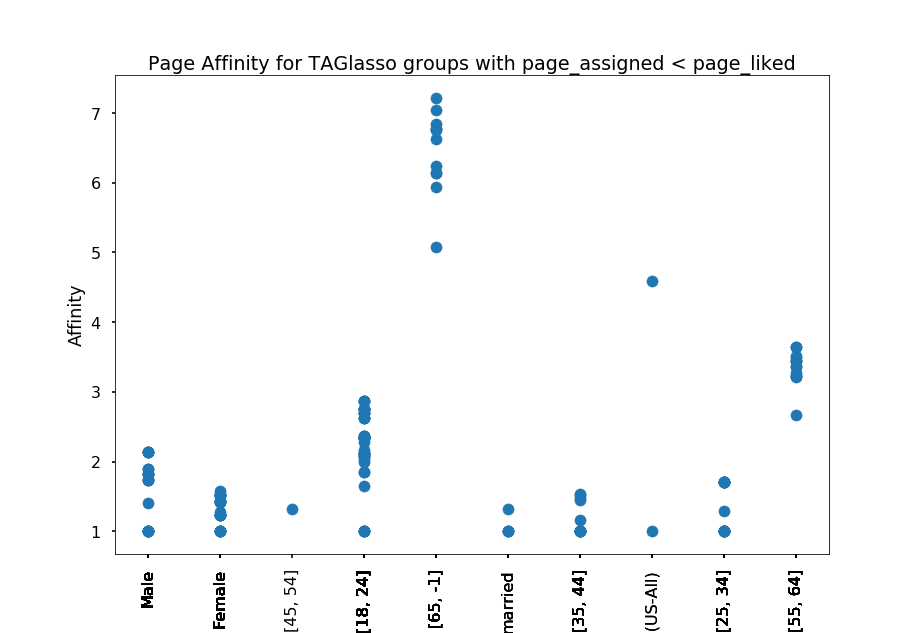
\includegraphics{images/affinity.png}
        \caption{Page affinities for pages that appear in TAGlasso hypotheses for each of the demographic values targeted by the same ad. The values on the x axis are demographic values uncovered by TAlasso run with demographic confounders explicitly added to the design matrix. Affinity is defined as the multiplicative probability that a user matching the demographic value will like the page compared to the baseline Facebook user.}
        \label{fig:affinity}
\end{figure}

Does time-adjusted group lasso signify the presence of confounder-based
targeting? \%\%\% End document

\printbibliography

\end{document}
